\section{Population sizes}

\begin{Figure}
  \centerfloat
     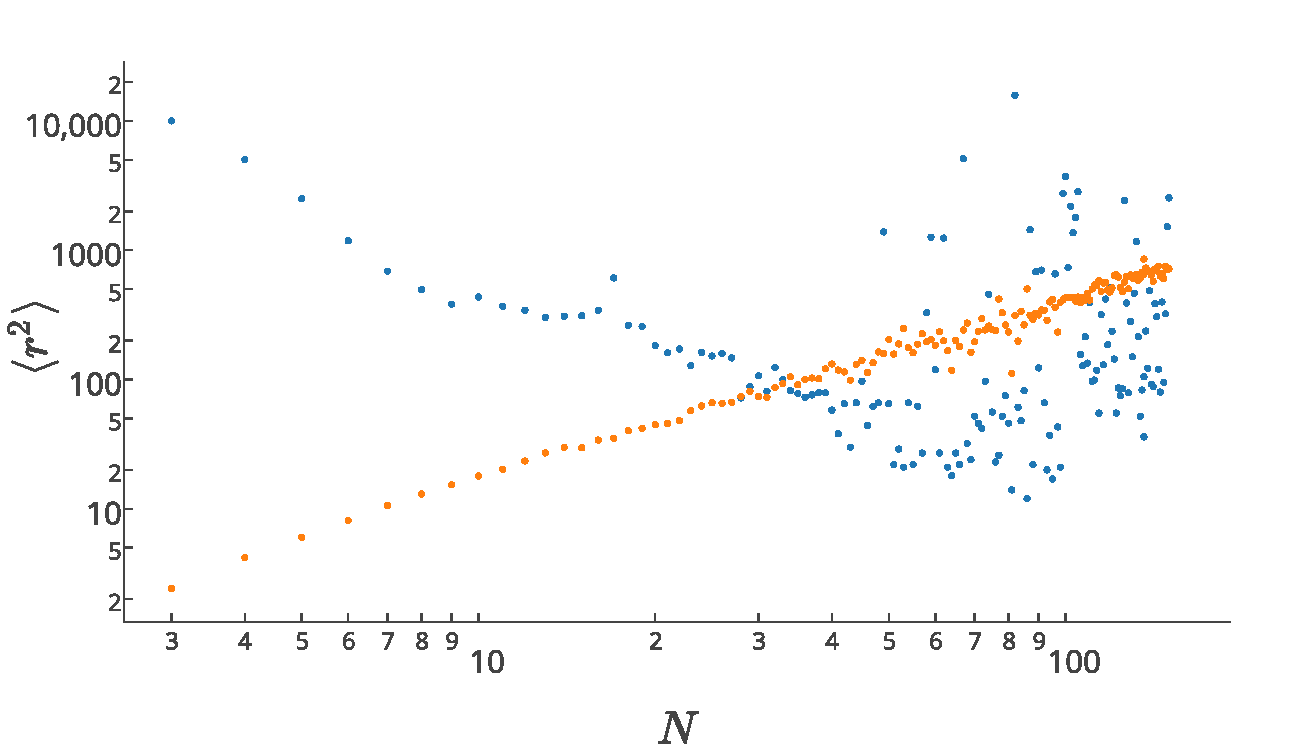
\includegraphics[width=\linewidth]{r_squared_pop.pdf}
 \captionof{figure}{End to end distance $\langle r^2 \rangle$ as function of polymer length $N_l$, with corresponding population sizes. The population size fluctuates a lot, especially for long polymers. This most likely influences the values found for $\langle r^2 \rangle$}\label{fig:r_squared_pop}
\end{Figure}
